\documentclass{article}
% Language setting
% Replace `english' with e.g. `spanish' to change the document language
\usepackage[english,russian]{babel}
\usepackage{amsmath}

%графика
\usepackage{wrapfig}
\usepackage{graphicx}
\usepackage{pgfplots}
\usepackage{tikz}


\usepackage{tcolorbox}

% Set page size and margins
% Replace `letterpaper' with `a4paper' for UK/EU standard size
\usepackage[letterpaper,top=2cm,bottom=2cm,left=3cm,right=3cm,marginparwidth=1.75cm]{geometry}

% Useful packages
\usepackage{amsmath}
\usepackage{amssymb}
\usepackage{graphicx}
\usepackage{fixltx2e}
\usepackage[colorlinks=true, allcolors=blue]{hyperref}

\usepackage{geometry}
\geometry{left=25mm,right=25mm,
 top=25mm,bottom=25mm}

\title{Количественная аналитика.\\
Лекции. Недели 1-2. \\
Прайсинг деривативов. Прайсинг опционов.}
\author{Синицын Павел}

% Колонтитулы
\usepackage{fancyhdr}
\pagestyle{fancy}
\renewcommand{\headrulewidth}{0.1mm}  
\renewcommand{\footrulewidth}{0.1mm}
\lfoot{}
\rfoot{\thepage}
\cfoot{}
\rhead{CMF-2022}
\chead{}

\begin{document}
\maketitle

% Оглавление
\setcounter{tocdepth}{1} % {2} - в оглавлении участвуют chapter, section и subsection. {1} - только chapter и section
\renewcommand\contentsname{Contents}
\tableofcontents
\newpage

% \section{Dictionary, Definitions, Abbreviations}

% \subsection{Dictionary}
% \begin{itemize}
%     \item IR - Interest rate - процентная ставка.
%     \item Compounding - платежи (idk)
% \end{itemize}

% \subsection{Definitions and Abbreviations}
% \begin{itemize}
%     \item SAR - Stated annual rate.
%     \item EAR - Effective annual rate.
%     \item FoC - Frequency of Compounding
%     \item PMT - Payment
%     \item r - Interest rate (at the moment). 
% \end{itemize}

\renewcommand{\labelitemi}{\tiny$\bullet$}
\renewcommand{\figurename}{Рис.}



 \section{Чем занимаются кванты}
\begin{itemize}
    \item Risk management (Управление рисками)
    \item Derivatives pricing models (Создание моделей ценообразования деривативов)
    \item Algorithmic strategies (Разработка алгоритмических стратегий)
    \item Optimal execution (Обеспечивает оптимальное исполнение)
    \item Asset allocation (Распределение активов)
\end{itemize}

\section{Типы квантов в деривативном прайсинге}
\begin{itemize}

  \item Model Implementation (Реализация моделей)
  
    \begin{itemize}
    \item Реализует модели ценообразования, непосредственно используемые трейдерами
    \item 80 процентов это написание кода
    \end{itemize}
   
   
  \item Model Governance (Управление моделями)
  
    \begin{itemize}
    \item Проводит независимую проверку моделей
    \item Запускает предоставленные скрипты
    \end{itemize}
   
  \item Model Research (Исследование моделей)


    \begin{itemize}
    \item Изобретает новые модели
    \item Исключительно математика
    \end{itemize}
    
\end{itemize}

\section{Виды работодателей}

\begin{itemize}
    \item Инвестиционные банки
    \item Хедж-фонды
    \item Коммерческие банки
\end{itemize}

\section{Классы активов}

\begin{itemize}

  \item FX (валютный обмен)
  
    \begin{itemize}
    \item Smile modelling (Моделирование улыбки)
    \item Большие объемы
    \item Sticky delta rule (Правило липкой дельты)
    \end{itemize}
   
  \item Акции
  
    \begin{itemize}
    \item Jump-diffusion (Прыжок-диффузия)
    \item Sticky strike rule (Правило липкого страйка)
    \end{itemize}
  

  \item Процентные ставки

    \begin{itemize}
    \item Самое сложное
    \item Основой является кривая
    \end{itemize}


  \item Сырьевые товары

    \begin{itemize}
    \item Высокая волатильность
    \item Зависимость от пути (усреднённых значений цены)
    \end{itemize}


  \item Кредитые деривативы (например CDS)
   
\end{itemize}

\section{Дополнительные свойства опциона}

\begin{itemize}

  \item Денежный поток
  
    \begin{itemize}
    \item Дивиденды/Купоны
    \end{itemize}
   
   
  \item Размерность
  
    \begin{itemize}
    \item Радуга
    \end{itemize}
   
  \item Зависимость от траектории


    \begin{itemize}
    \item Сильная - азиатский опцион
    \item Слабая - барьерный опцион
    \end{itemize}

  \item Встроенные решения


    \begin{itemize}
    \item Американские/бермудские опционы
    \end{itemize}

  \item Базовая модель
   
\end{itemize}

\section{Языки программирования для прайсинга деривативов}

\begin{itemize}

  \item С++
  
    \begin{itemize}
    \item Возможность многократного использования
    \item Эффективность
    \end{itemize}
   
   
  \item Python/MATLAB/R
  
    \begin{itemize}
    \item Прототипирование
    \item Подготовка данных
    \item Визуализация
    \end{itemize}

\end{itemize}

\section{Общая структура прайсинга деривативов}

\begin{itemize}
 
  \item Дериватив
  \item Базовая модель
  \item Список дополнительных свойств
  
    \begin{itemize}
    \item Finite-difference scheme (Конечно-разностная схема)
    \item Closed-form solution (Решение в закрытой форме)
    \item Метод Монте-Карло
    \end{itemize}

\end{itemize}
\section{План курса}
  
\begin{itemize}
 
  \item Математический бэкграунд. Основные результаты. PDE против нейтрального к риску подхода. Методы оценки греческих коэффициентов.
  \item Ванильные продукты. Вывод решения в закрытой форме. Происхождение греков в закрытой форме. Реализация на С++.
  \item Дополнительные деривативы. Пример продукта (досрочное осуществление прав). Возможные решения. Конечно-разностные схемы - обзор, основные результаты.
  \item Конечно-разностные схемы - дополнительные темы. Добавление в продукт новых функций, обсуждение эффективности.
  \item Дополнительные деривативы. Пример продукта (сильная зависимость от траектории). Возможные решения. Методы Монте-Карло - обзор, основные результаты.
  \item Методы Монте-Карло - дополнительные темы. Измените программу, уменьшите дисперсию, сравните эффективность.

\section{Приложения}

\begin{figure}[h]
\centering
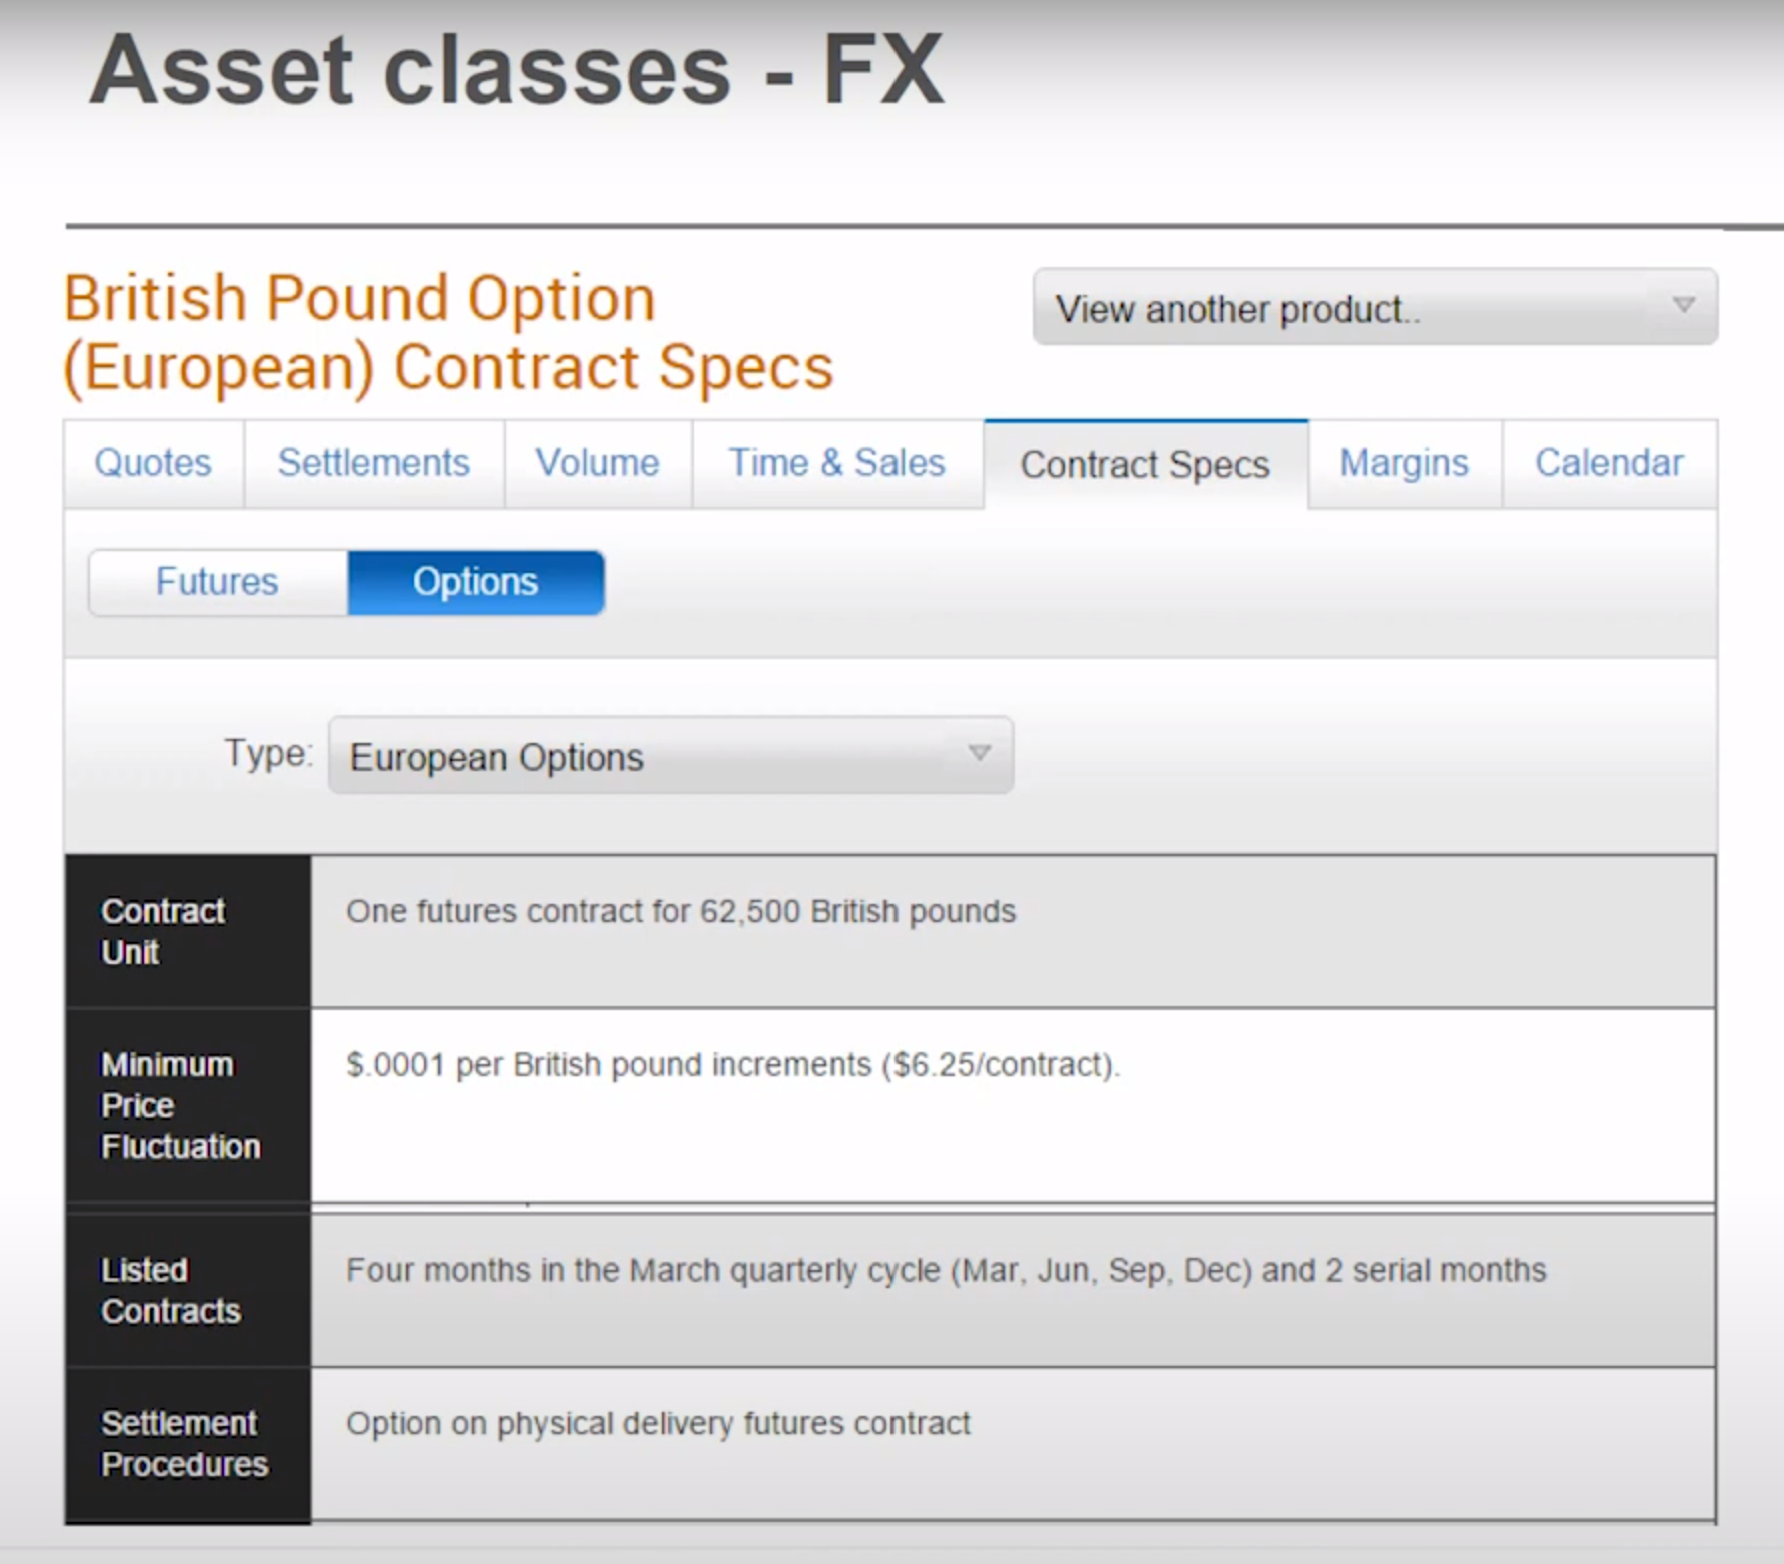
\includegraphics[width=0.7\textwidth]{1.png}
\caption{Пример FX}
\label{loadings}
\end{figure}

\begin{figure}[h]
\centering
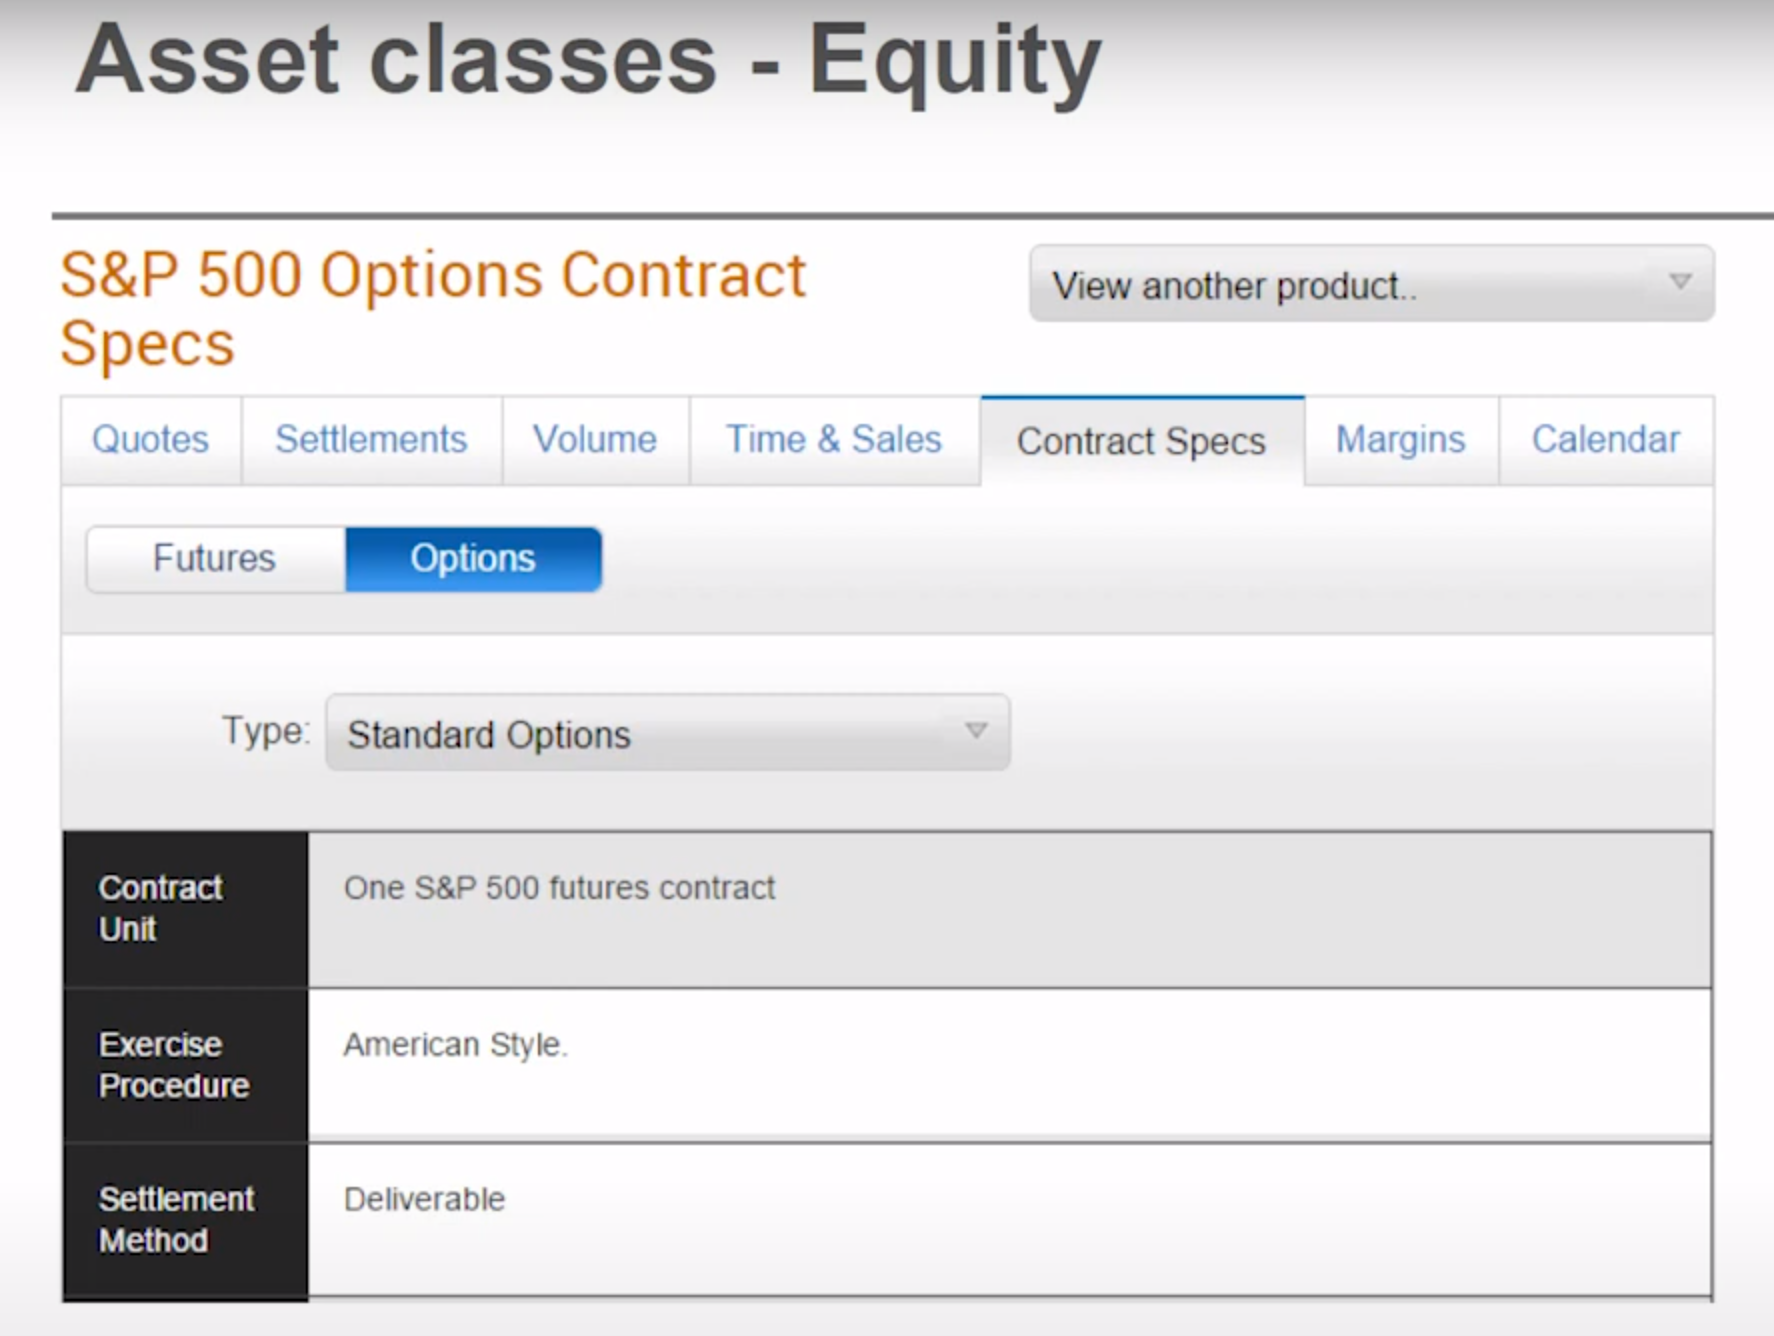
\includegraphics[width=0.7\textwidth]{2.png}
\caption{Пример Equity}
\label{loadings}
\end{figure}

\begin{figure}[h]
\centering
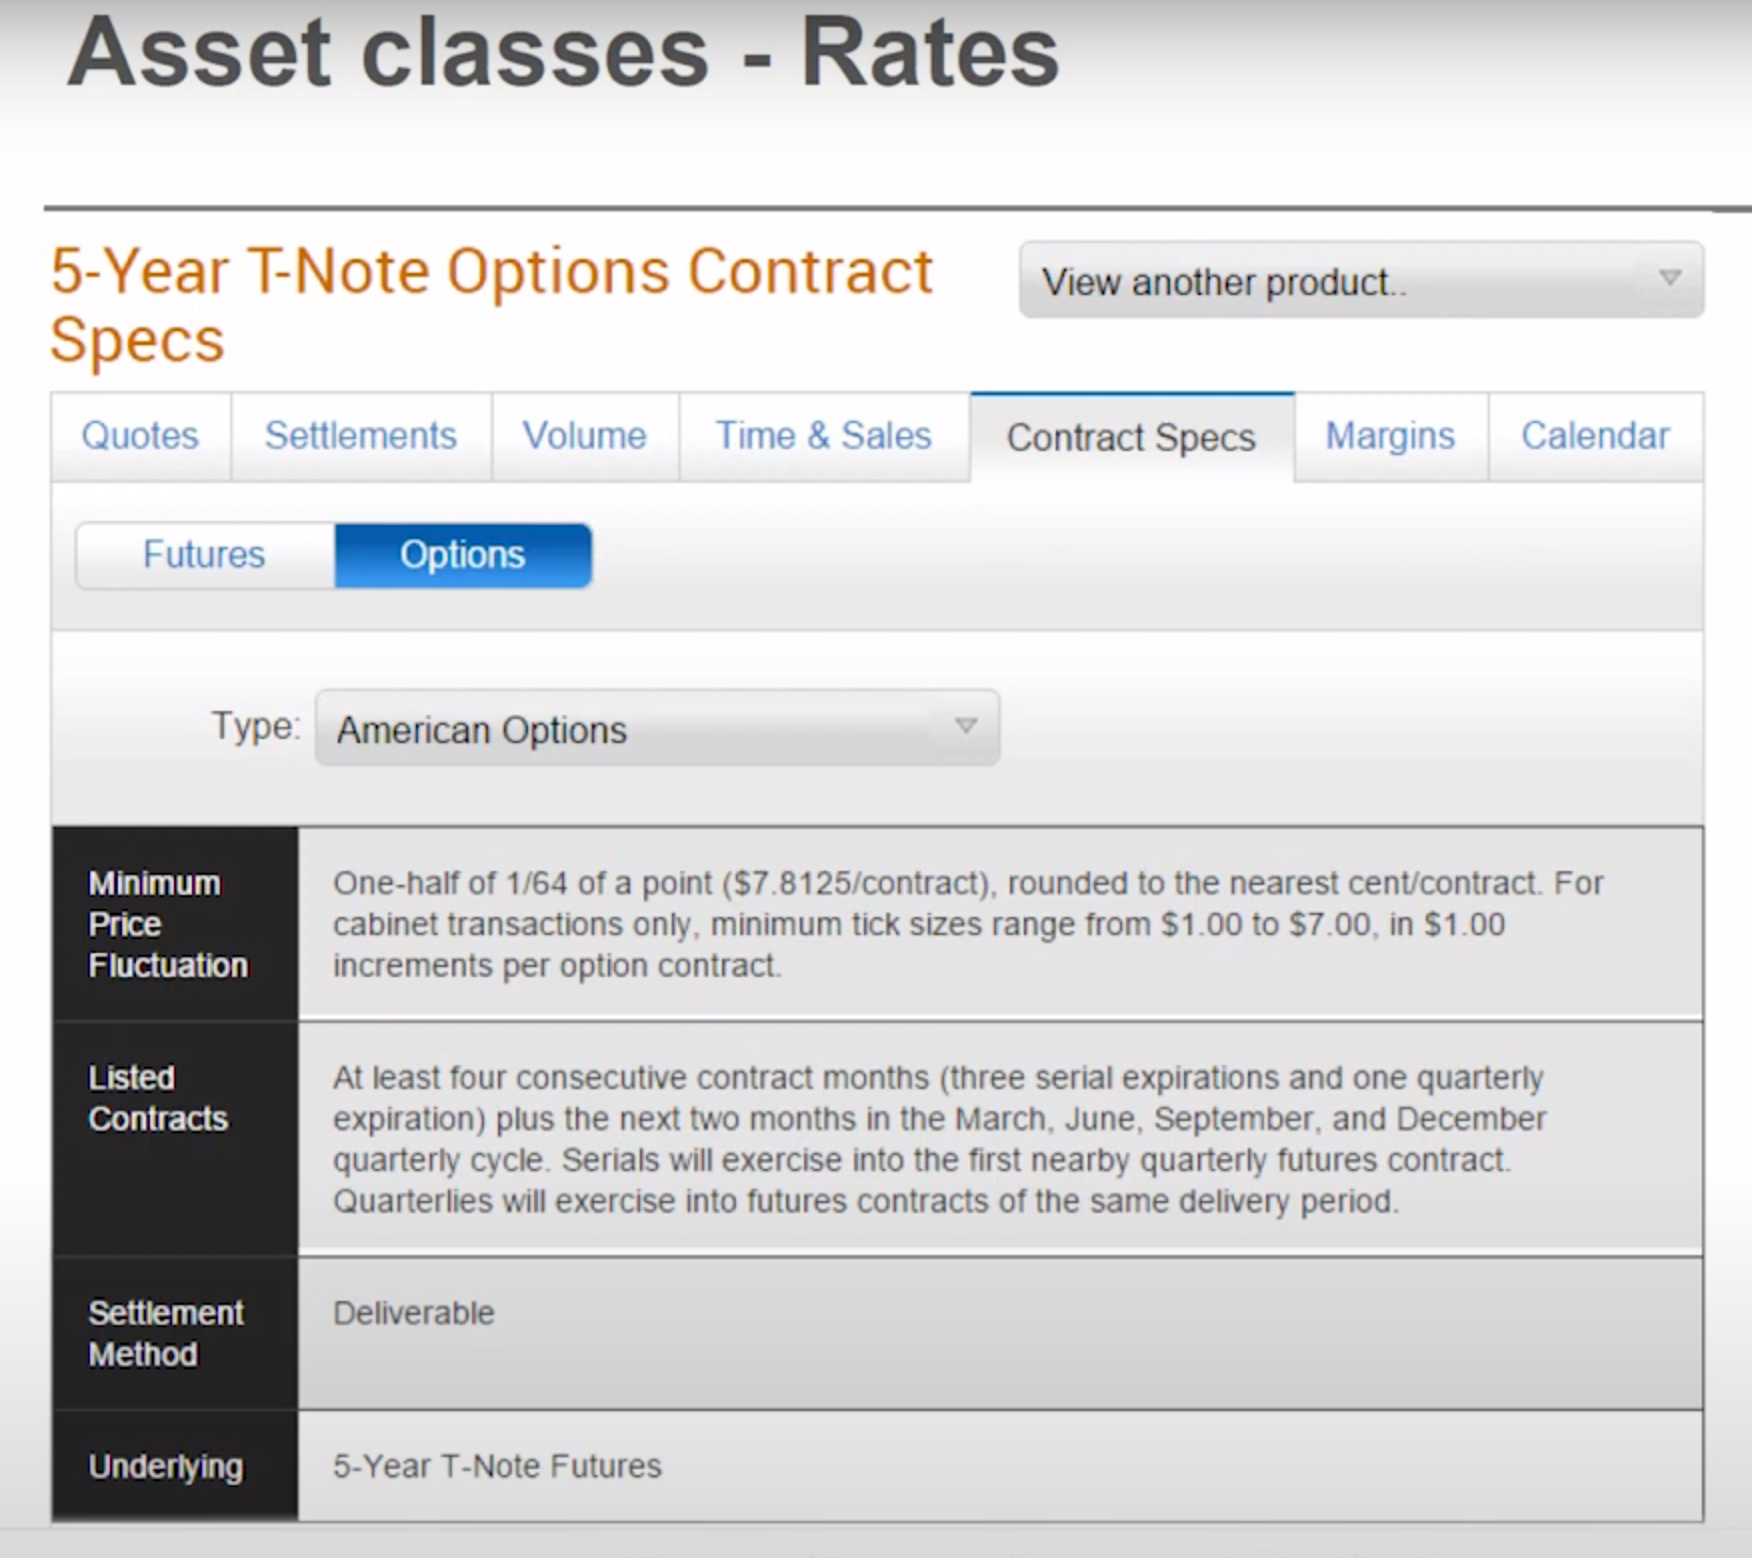
\includegraphics[width=0.7\textwidth]{3.png}
\caption{Пример Rates}
\label{loadings}
\end{figure}

\begin{figure}[h]
\centering
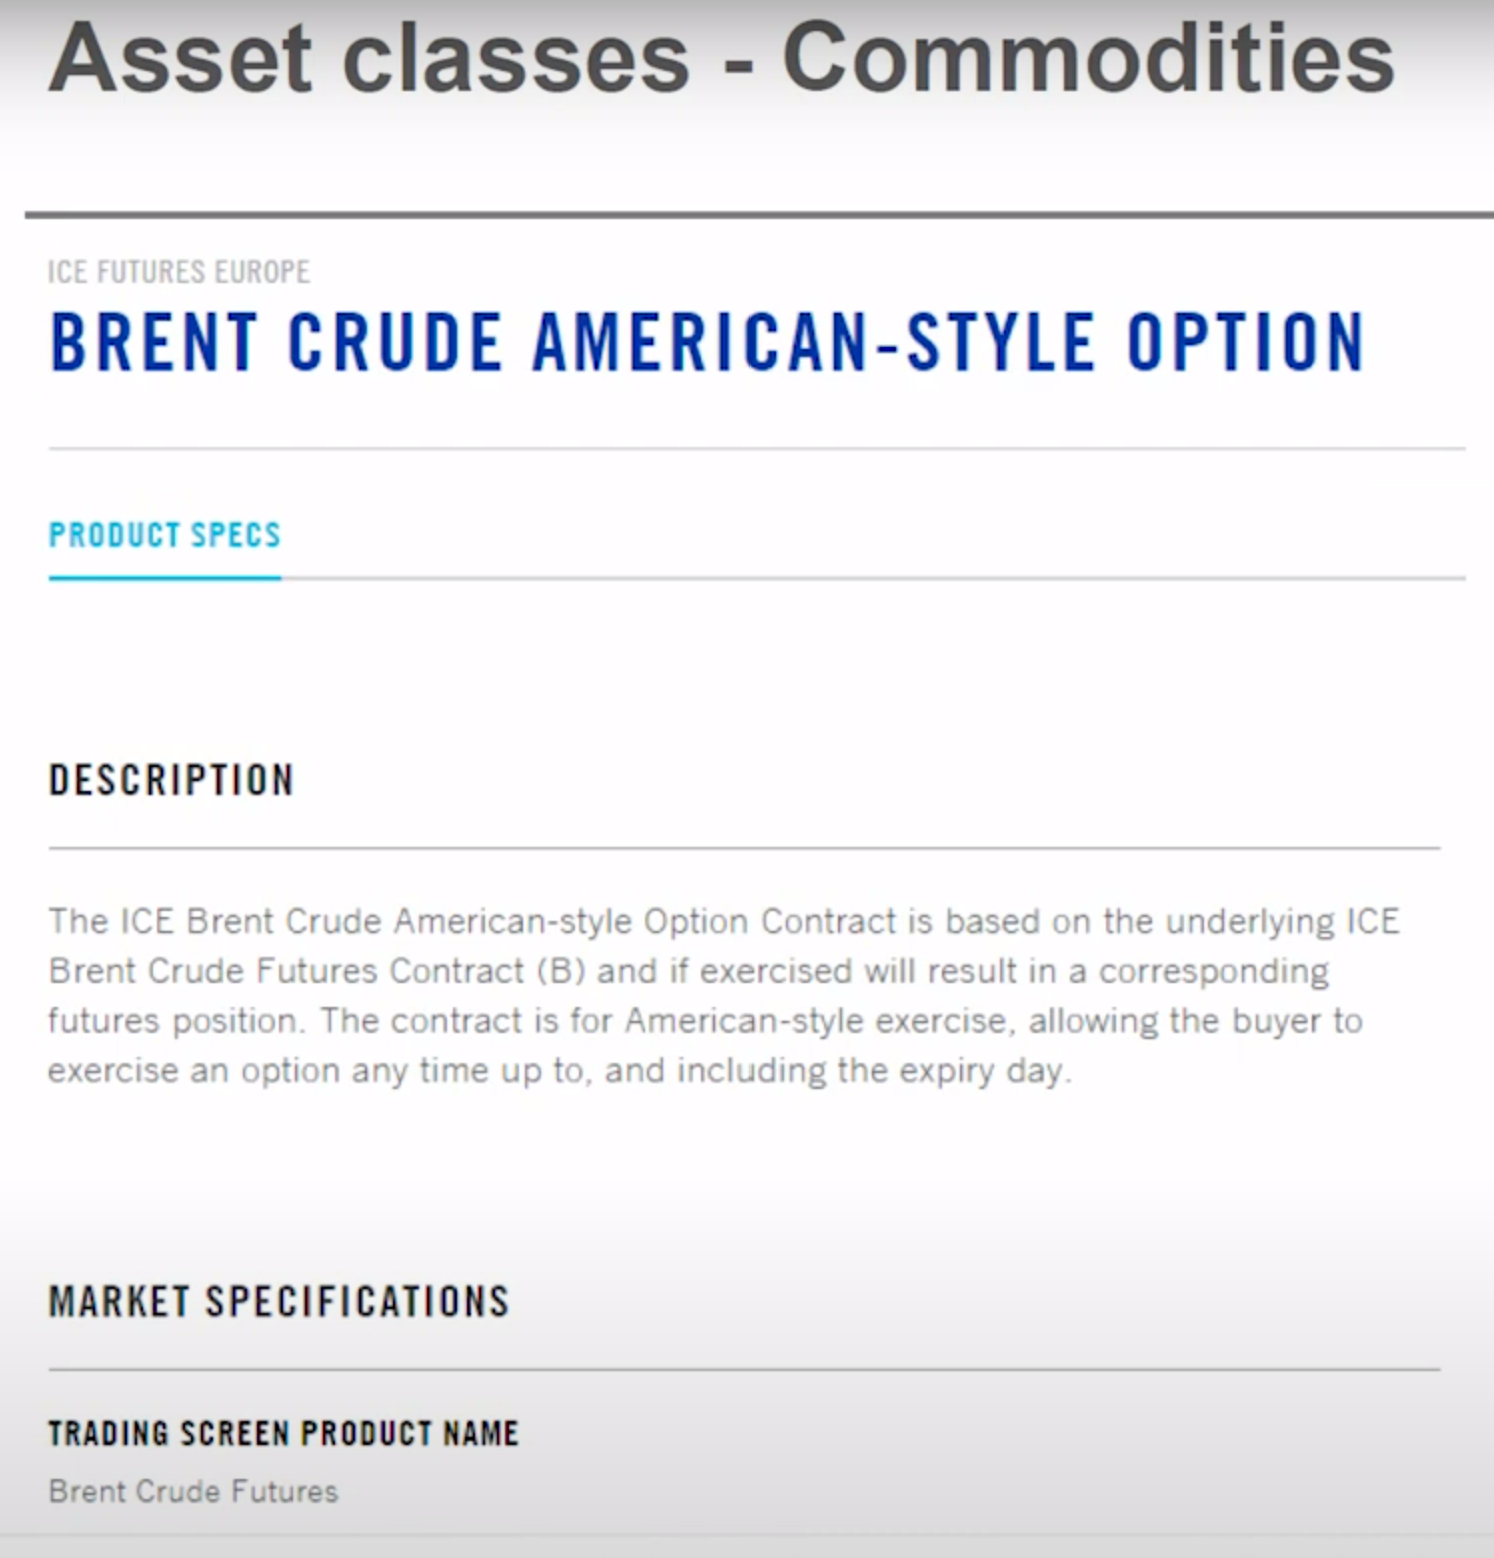
\includegraphics[width=0.7\textwidth]{4.png}
\caption{Пример Commodities}
\label{loadings}
\end{figure}

\begin{figure}[h]
\centering
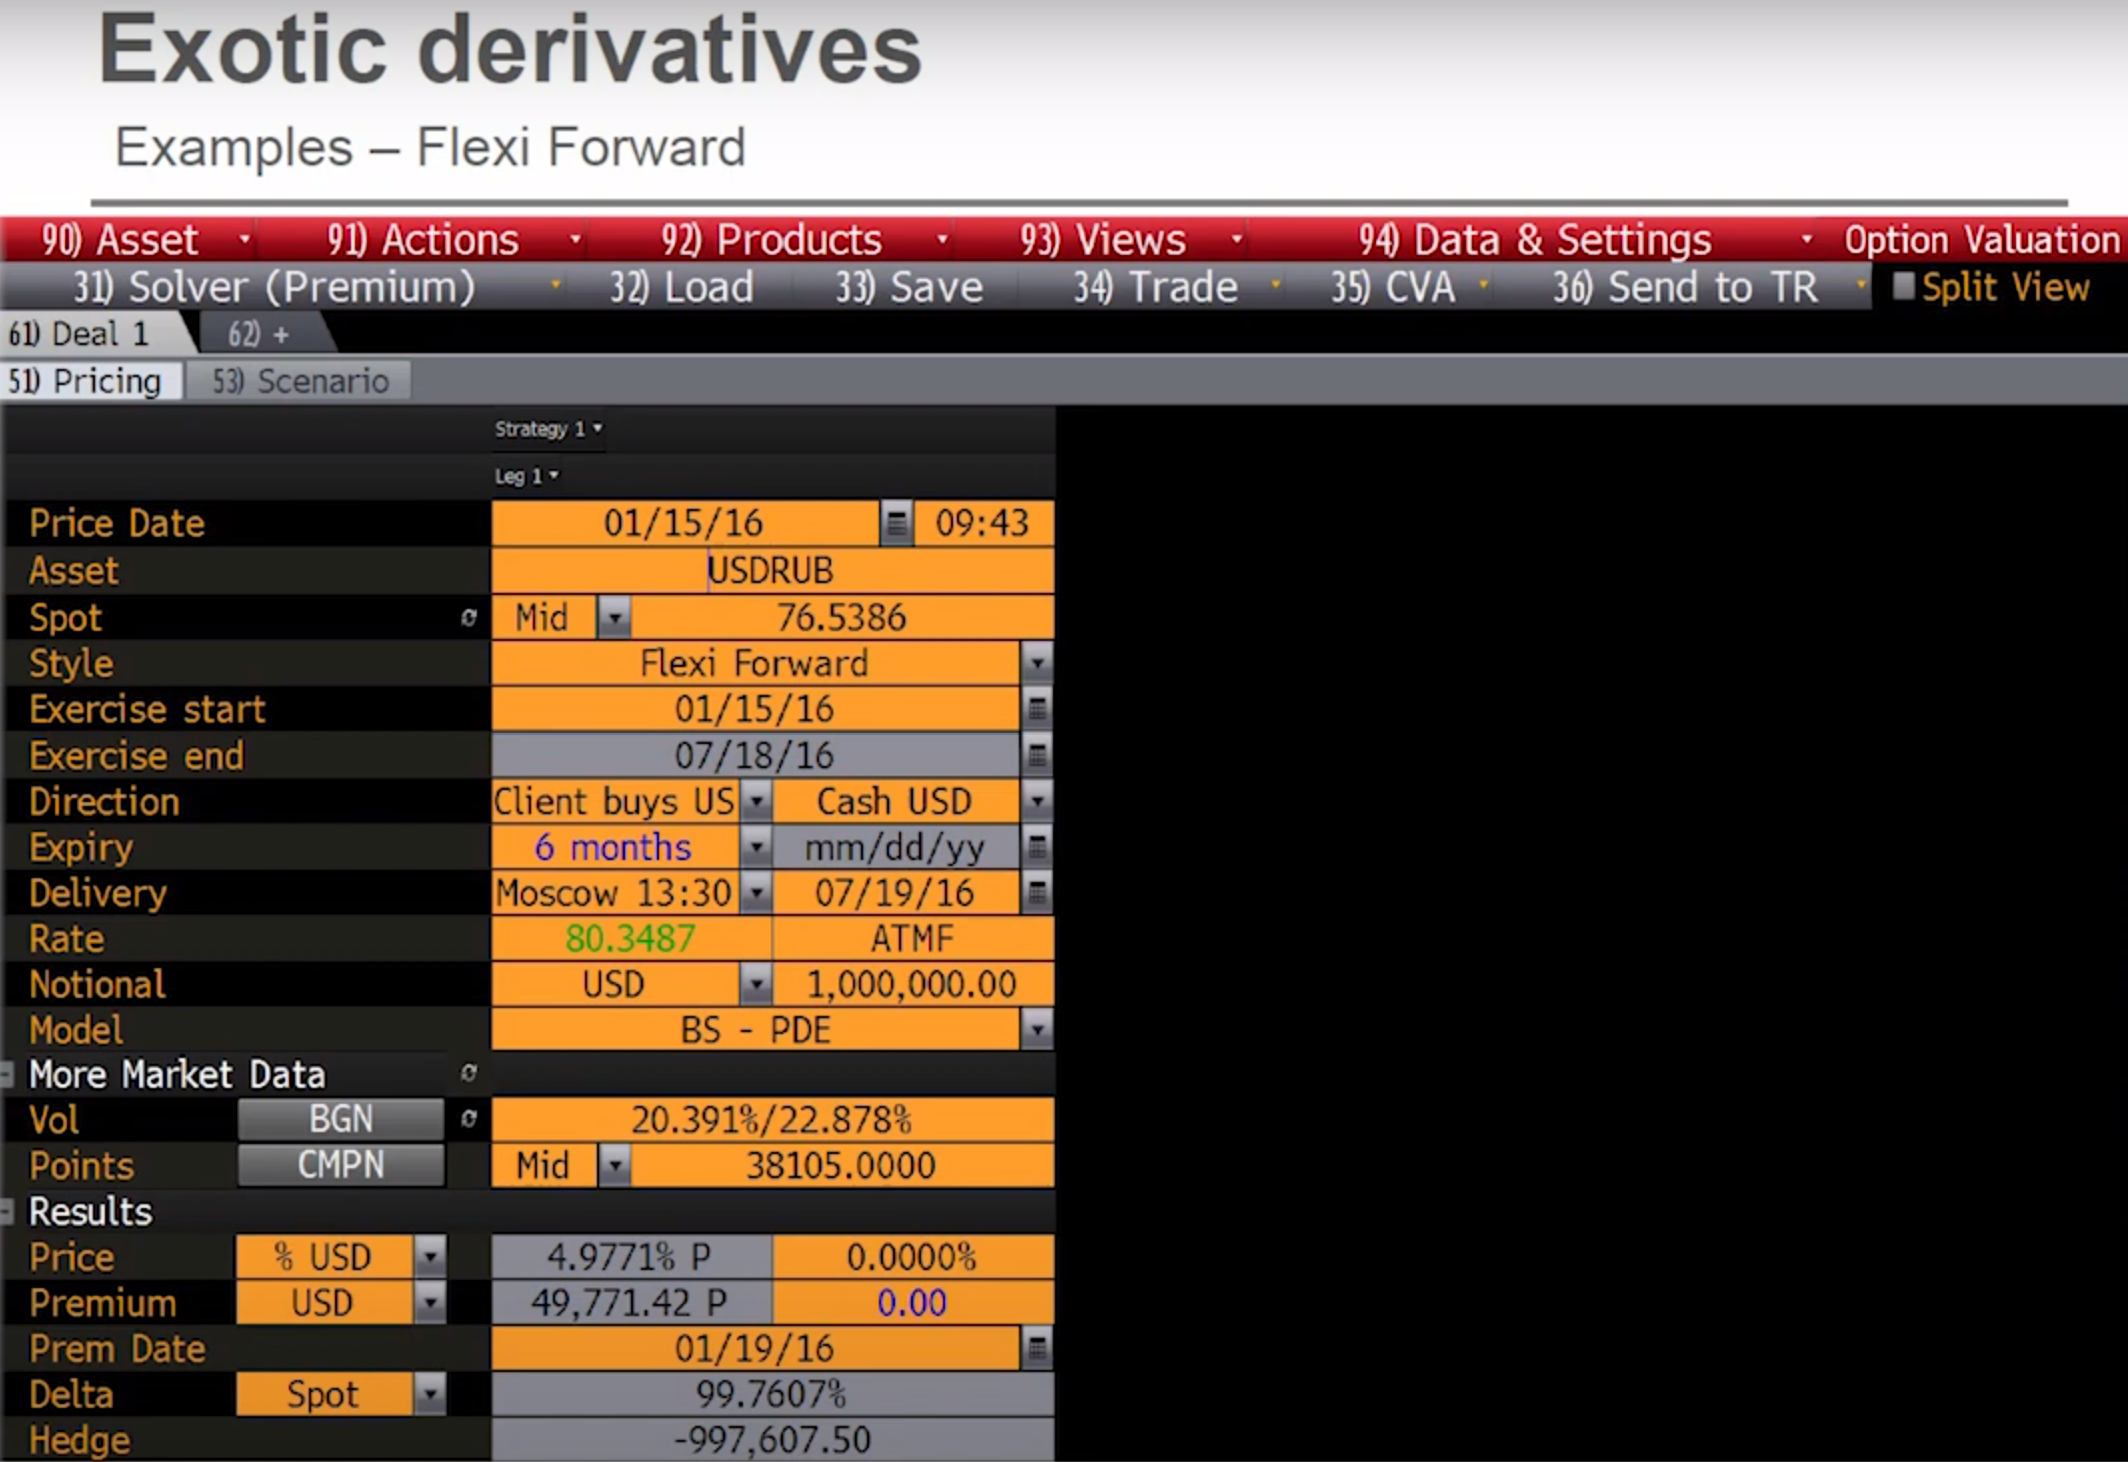
\includegraphics[width=0.7\textwidth]{5.png}
\caption{Пример Flexi Forward}
\label{loadings}
\end{figure}


\begin{figure}[h]
\centering
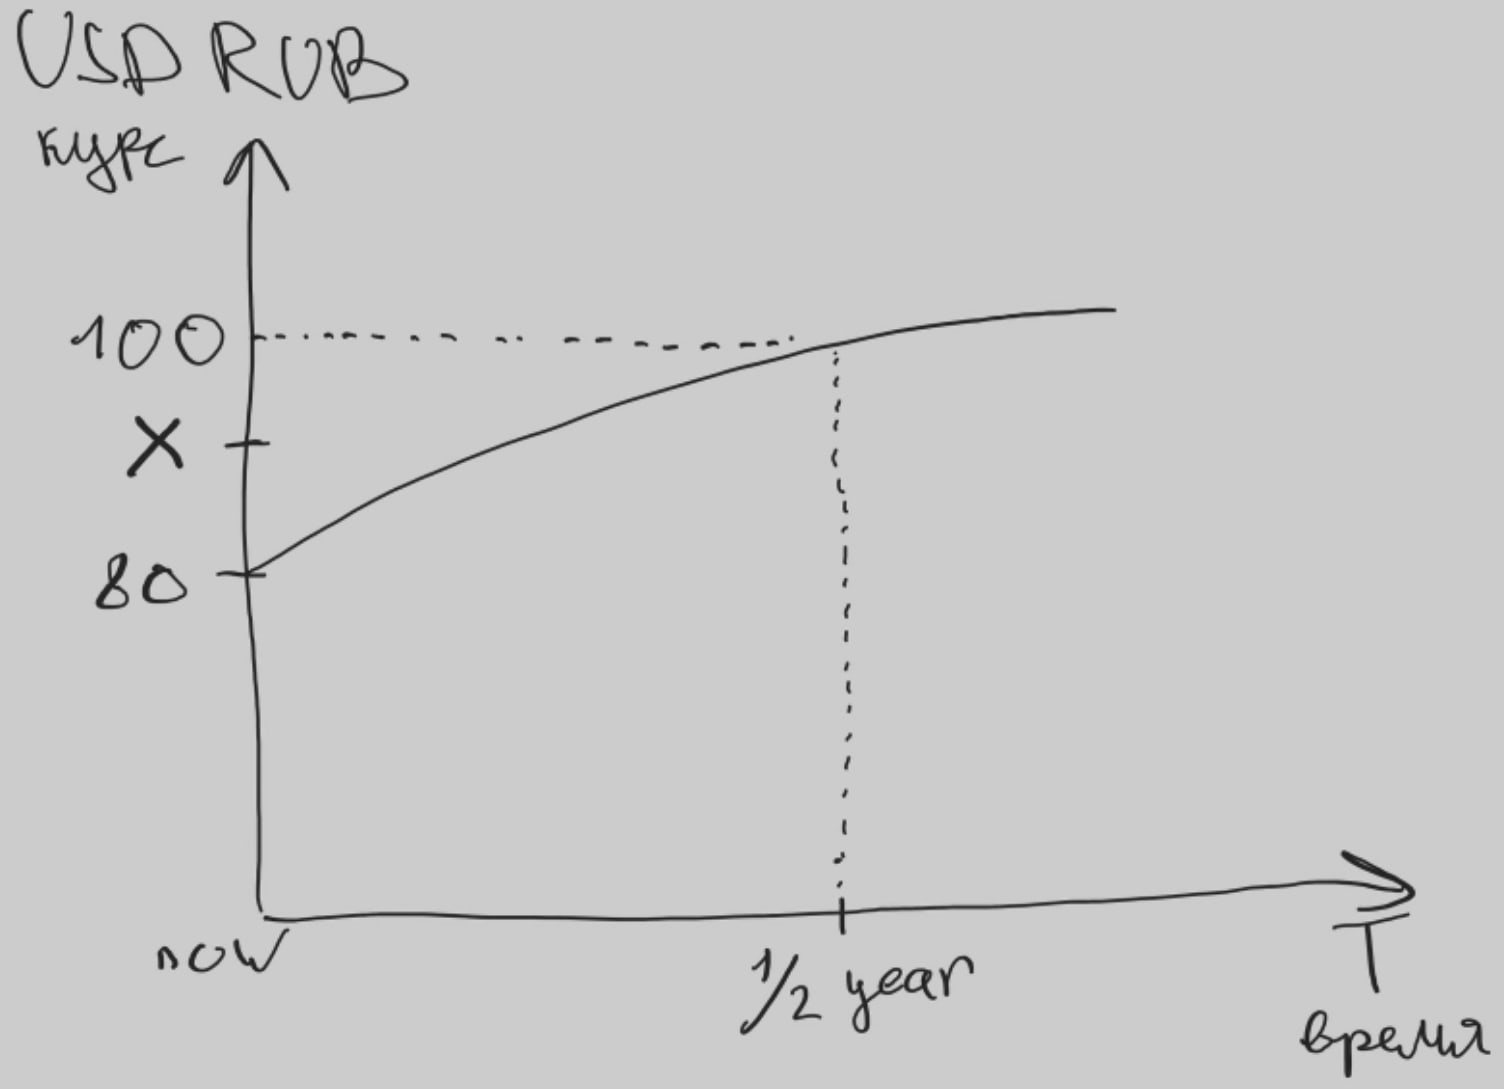
\includegraphics[width=0.7\textwidth]{7.png}
\caption{График}
Как через полгода купить/продать фьючерс по цене X? Как выбрать цену X?

Непонятно в какой момент клиент исполнит. Поэтому мы можем оказаться с незахеджированной позицией. Из-за этого цену непросто определить.
\label{loadings}
\end{figure}


\begin{figure}[h]
\centering
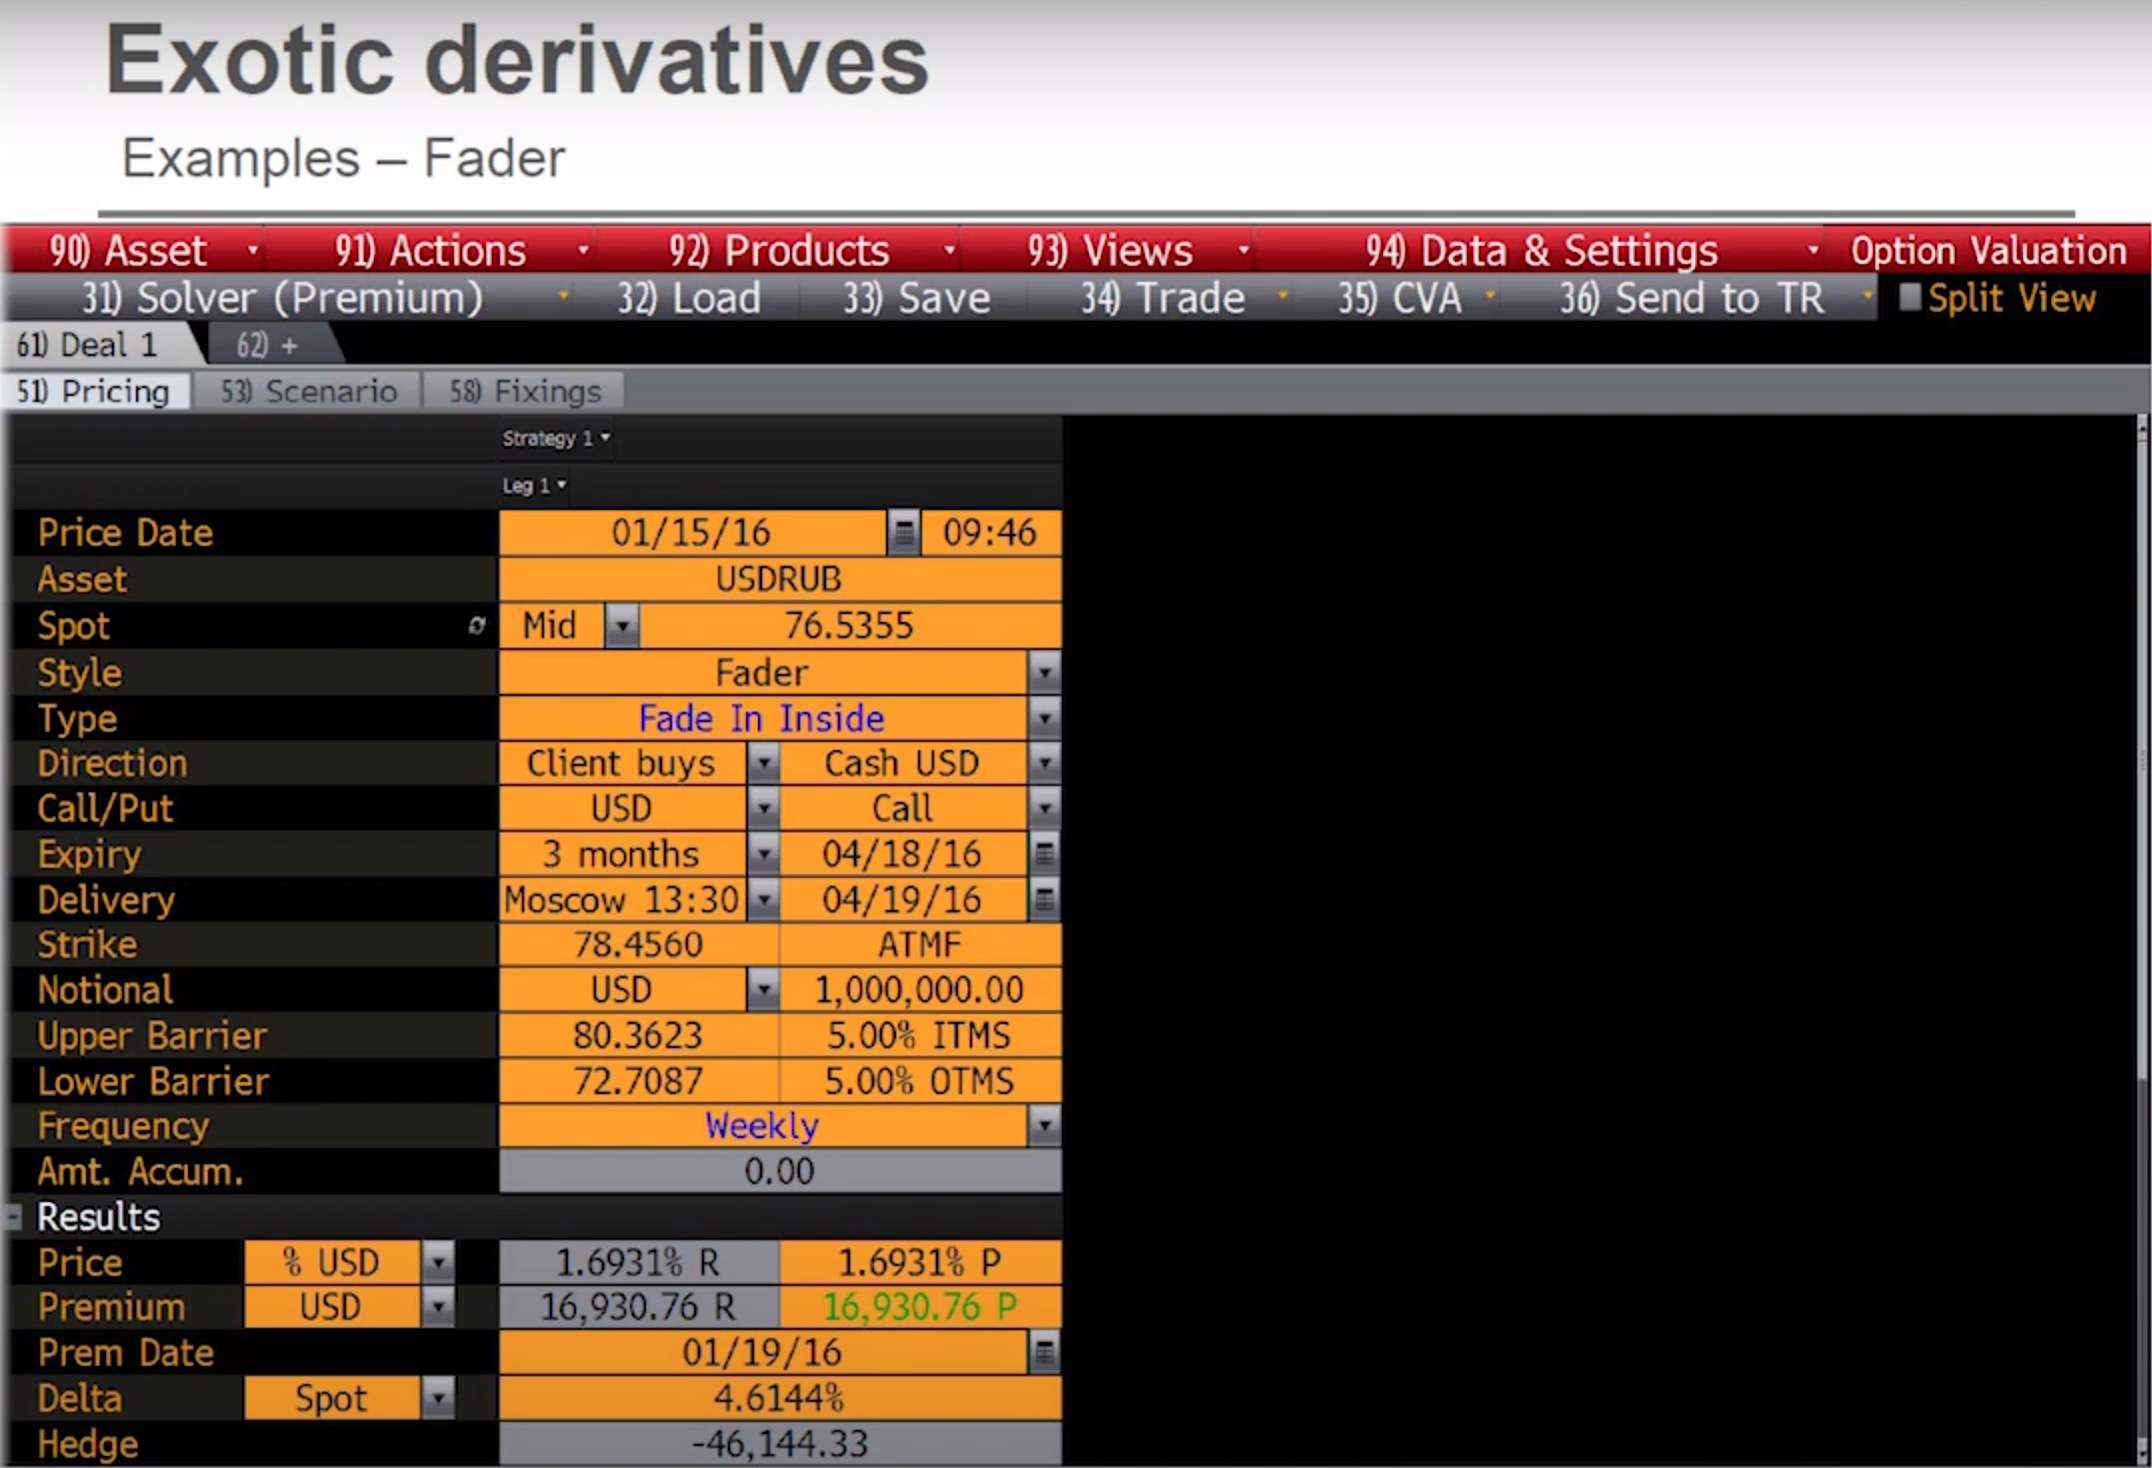
\includegraphics[width=0.7\textwidth]{6.png}
\caption{Пример Fader}
\label{loadings}
\end{figure}


\end{itemize}
\end{document}